%!TEX root=../ast2016.tex

\begin{figure*}[t]
  \centering
  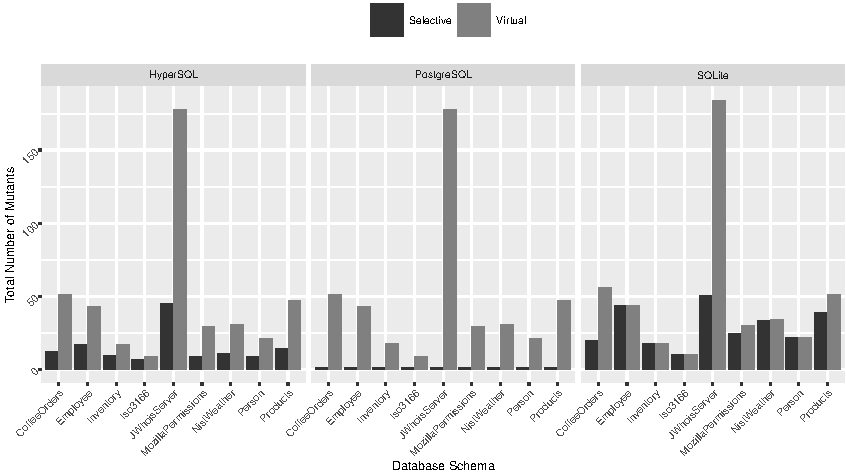
\includegraphics[scale=1.0]{graphics/graphic_barplot_schema_mutantcount_vm_tcm.pdf}
  \caption{Box plot of the mutation score for the virtual and time-constrained mutation analysis techniques.}

  {\small \justifying{ \noindent In this plot the height of the bar corresponds to the number of mutants subject to
      analysis by the virtual and time-constrained methods; this count is reported for all of the chosen relational
      schemas and the three database management systems. Since the time-constrained technique employs randomness to
      select mutants that can be run within a specified time limit, the height of a light grey bar is the average across
      a total of thirty runs; virtual mutation analysis is deterministic and thus the height of the dark grey bar is a
      direct count. } \par}

\end{figure*}
